\section{Proposed technical architecture and challenges (RQ4)}~\label{section:technical_architecture}
As an organization covering areas like research, student affairs and administration a university has to manage a significant amount of knowledge, adding new information on a daily basis.
Such an application domain is complex and includes areas like management of an academic library and provision of educational resources which have to be conform to stakeholders requirements. Traditionally the \textit{Service Oriented Architectures~(SOA)} have been used to meet these needs. However, as the application domain grows many small and similar services tend to emerge. That phenomena cannot only be observed at the Vienna University of Technology, but also at the Open University\footnote{\url{http://www.open.ac.uk/}}~\citet{inproceedings:zablith_consuming_2011}.

A major problem of evolving similar, independent services are diverging data formats and service owners. Thus, knowledge and administrative information that has been collected by multiple services can not be easily interlinked. An example for such isolated services is the e-learning platform called TUWEL\footnote{\url{https://tuwel.tuwien.ac.at/}}, combining moodle\footnote{\url{https://moodle.org/}} and the central information system called TISS\footnote{\url{https://tiss.tuwien.ac.at/}}. These services provide course information and material, but are intended for different purposes. Whereas TISS focuses mainly on administrative functionality, TUWEL supports the interaction between teacher and student. 
Adding additional services which, for example, synchronize deadlines and registration dates is costly due to the fact that the information is separated over different isolated sources and not easily accessible. 

\subsection{The big picture: a publication framework}~\label{section:publication_framework}

\begin{figure}[htbp]
\centering
{\scalebox{0.7}{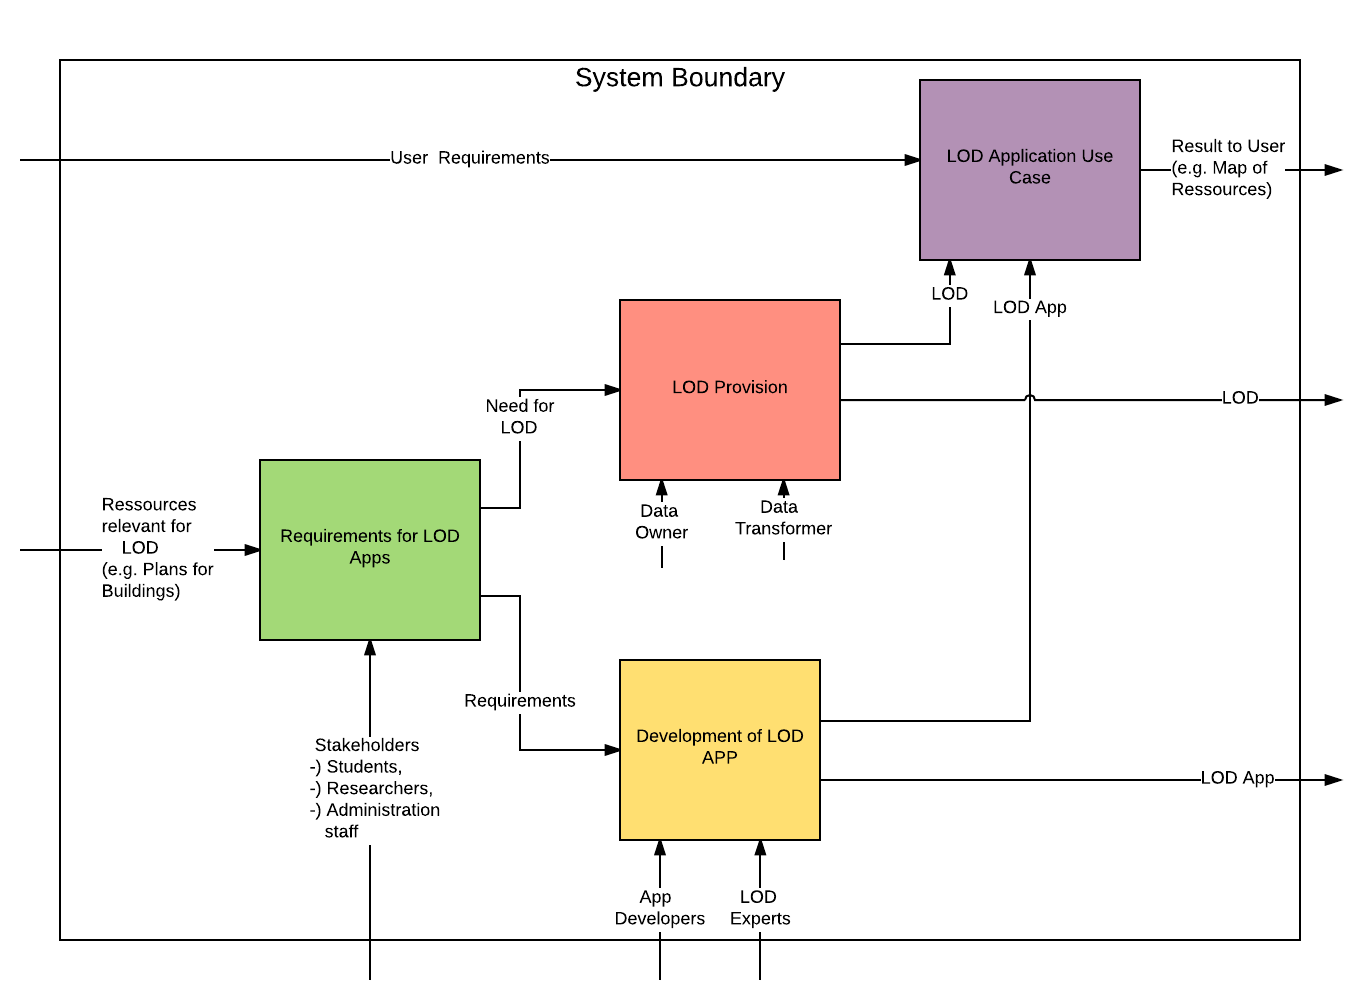
\includegraphics{images/architecture/idef0.png}}}
\caption[High level framework for LOD publishing]{High level framework for LOD publishing in IDEF0 notation}
\label{Fi:idef0}
\end{figure}
\subsubsection{Parts}
In this sub-section we provide an overview of a high level architecture, illustrated in Figure~\ref{Fi:idef0}, for a university wide publication framework which includes:

\begin{itemize}
	\item \textbf{Requirements for LOD-Applications}\newline
	At the beginning stand the existing resources and the needs of the stakeholder. Combining these leads to the requirements for an application, the first step of the process. According to this requirement a decision has to be made whether they are realizable depending on the cost-value ratio and whether the solution has to be a LOD application. These process has to actively involve all stakeholders.
	\item \textbf{Data Provision}\newline
	After defining the requirements, the existing data (e.g. a publication database) must be transformed in a appropriate, machine readable LOD format. These can happen in a manually (only for small data sets) or a (semi-)automated (for big data set) way. Ideally there is a automated transformer based on an existing, well maintained and up-to-date database so there has to be less cared about the of the data (for a more technical description see Section~\ref{subsubsec:sources}). Key roles for this process are the original data owner and the data transformer.
	\item \textbf{Development of an Application}\newline
	Based on the requirements definitions from the previous step a proper application (e.g. a browser of publication data) now can be constructed considering the stakeholder needs and existing resources (transformed to LOD).  To support this process and to not obtaining all knowledge from zero it is recommended to access the knowledge of LOD experts (e.g. provided by the LinkedUniversities~\footnote{\url{www.linkeduniversities.org/}}). The development can simultaneously be done with the data provision if proper interface between the application and its data are made. 
	\item \textbf{Application Use Case}\newline
	Combining the data, transformed in LOD, the LOD application and user requirements (not the application requirements from the first step) result in the actual application use case, representing the environment or the domain.
\end{itemize}

\subsubsection{In- and outbound interfaces}

There were several indirectly interfaces mentioned above - we define them now in a more formal way and divide them in inbound (arrows pointing from outside the system boundary) and outbound interfaces (arrows pointing from inside the system boundary).

The inbound interfaces are:

\begin{itemize}
	\item \textbf{User Requirements}\newline
	Understanding user requirements is an essential part of the software development process. Due to the open nature of Linked Open Data privacy concerns and legal issues should be already considered in the requirements as misunderstandings are hard to fix in later phases.
	\item \textbf{Existing Resources}\newline
	The starting point of every LOD application are resources, ideally already existing (to reduce the amount of work). It can be everything from relational databases, simple Excel files or other Linked (Open) Data sets. For more details see section~\ref{subsubsec:sources}.
	\item \textbf{Stakeholders}\newline
	Stakeholders are defined as \textit{``a person, group or organization that has interest or concern in an organization. Stakeholders can affect or be affected by the organization's actions, objectives and policies.''}~\citet{book:Post2002} Their needs and demands have to be considered in a LOD project as similar as in every other software project.
	\item \textbf{Application Developers}\newline
	\item \textbf{LOD Experts}\newline
	To avoid unnecessary redundancy in acquiring knowledge of LOD implementation, it is highly recommended to involve either LOD experts in the development or access their accumulated know-how e.g. by platforms like LinkedUniversities~\footnote{\url{www.linkeduniversities.org/}} (see section~\ref{linkeduniversities})
	\item \textbf{Data Owner}\newline
	Every data set has its owner, therefore this role has to be considered in the development process to avoid organizational conflicts and copyright issues. Ideally he is directly involved to access his specific know-how about the data set.
	\item \textbf{Data Transformer}\newline
	To use a data set in a LOD approach, the data have to be transformed either manually or (semi-)automatically into a proper format (see~\citet{article:bernerslee_2006} for the 5 star model of data format and section~\ref{subsubsec:sources} for details about transformations).
\end{itemize}

The outbound interfaces are:

\begin{itemize}
	\item \textbf{Linked Open Data}\newline
	As a result of the LOD provision the actual data are provided e.g. as SPARQL endpoint, so others can easily access and use them in other applications. For technical details about endpoints see section~\ref{subsubsec:provision} or as example the SPARQL endpoint of The Open University~\url{www.data.open.ac.uk/query}.
	\item \textbf{Application}\newline
	The outcome of the development phase are applications for end-users to access and interact with the data e.g. in form of a web platform. For technical details about endpoints see section~\ref{subsubsec:provision} or as example the application list of The Open University~\url{www.data.open.ac.uk/applications.html}.
	\item \textbf{End-User Result}\newline
	Finally the main result is the actual interaction of the users with the applications and endpoints, (hoepfully) acting in the boundaries of the defined use cases.
\end{itemize}

\newpage

\subsection{Proposal of a technical architecture}~\label{subsection:proposal_technical_architecture}

In order to overcome the environment of data silos and to support the evolvement of a university-wide data space for public resources, a technical architecture following Linked Data principles is proposed and discussed in this section. Berners-Lee suggested four principles for publishing data on the web, which can be considered as best practise. The compliance with this best practise leads to Linked Data; \enquote{the idea is that the more people follow these principles, the more their data will be usable by others.}\cite{simperl_using_2013}. The four principles stated by Berners-Lee (2006)~\cite{article:bernerslee_2006} are:
\begin{enumerate}
	\item Use URIs as names for things
	\item Use HTTP URIs so that people can look up those names.
	\item When someone looks up a URI, provide useful information, using the standards (RDF, RDFS, SPARQL)
	\item Include links to other URIs. so that they can discover more things.
\end{enumerate}

Linked Open Data extends Linked Data with the idea of publishing it in a open way.
\begin{quote} Open means anyone can freely access, use, modify, and share for any purpose (subject, at most, to requirements that preserve provenance and openness).\cite{url:open_definition}\end{quote}

In order to transform demanded datasets of the university into Linked Data and publish it in an open way, a system architecture is required that faces the issues of diverging data sources and data freshness.\enquote{An important architectural pattern used in system development is the multitier architecture. It logically separates the functionality of the system in a number of layers and specifies the communication between those layers.}\cite{simperl_using_2013}.

%In this section we will briefly describe a proposal technical architecture for publishing %(existing) data as Linked Open Data
% with the help of the example use case ``publication data as LOD'' (see section~\ref{section:pub_db_usecase})
. 

The proposed architecture is mainly inspired by the toolkit ``\texttt{Tabloid}'' (``Toolkit ABout Linked Open Institutional Data'') by the LUCERO Project~{\footnote{\citet{url:lucero-tabloid}} - a collection of tools, examples and documentations. The general principle is a system, which extract RDF data from existing data sources (section~\ref{subsubsec:sources}), load them into a triple store (section~\ref{subsubsec:store}) and finally expose them to the web (section~\ref{subsubsec:provision}). For illustration see the LUCERO workflow in figure~\ref{Fi:lucero_architecture} (in this part only the generic parts are described). In this workflow there are way more components than we will talk about (e.g. mechanism of detecting data changing) than shown in the figure. Additional a more generic architecture can be seen in figure~\ref{Fi:tec_architecture}.
%url:linked-universities-vocabularies
%url:linked-universities-tools
%url:lucero-tabloid

\begin{figure}[htbp]
\centering
{\scalebox{0.5}{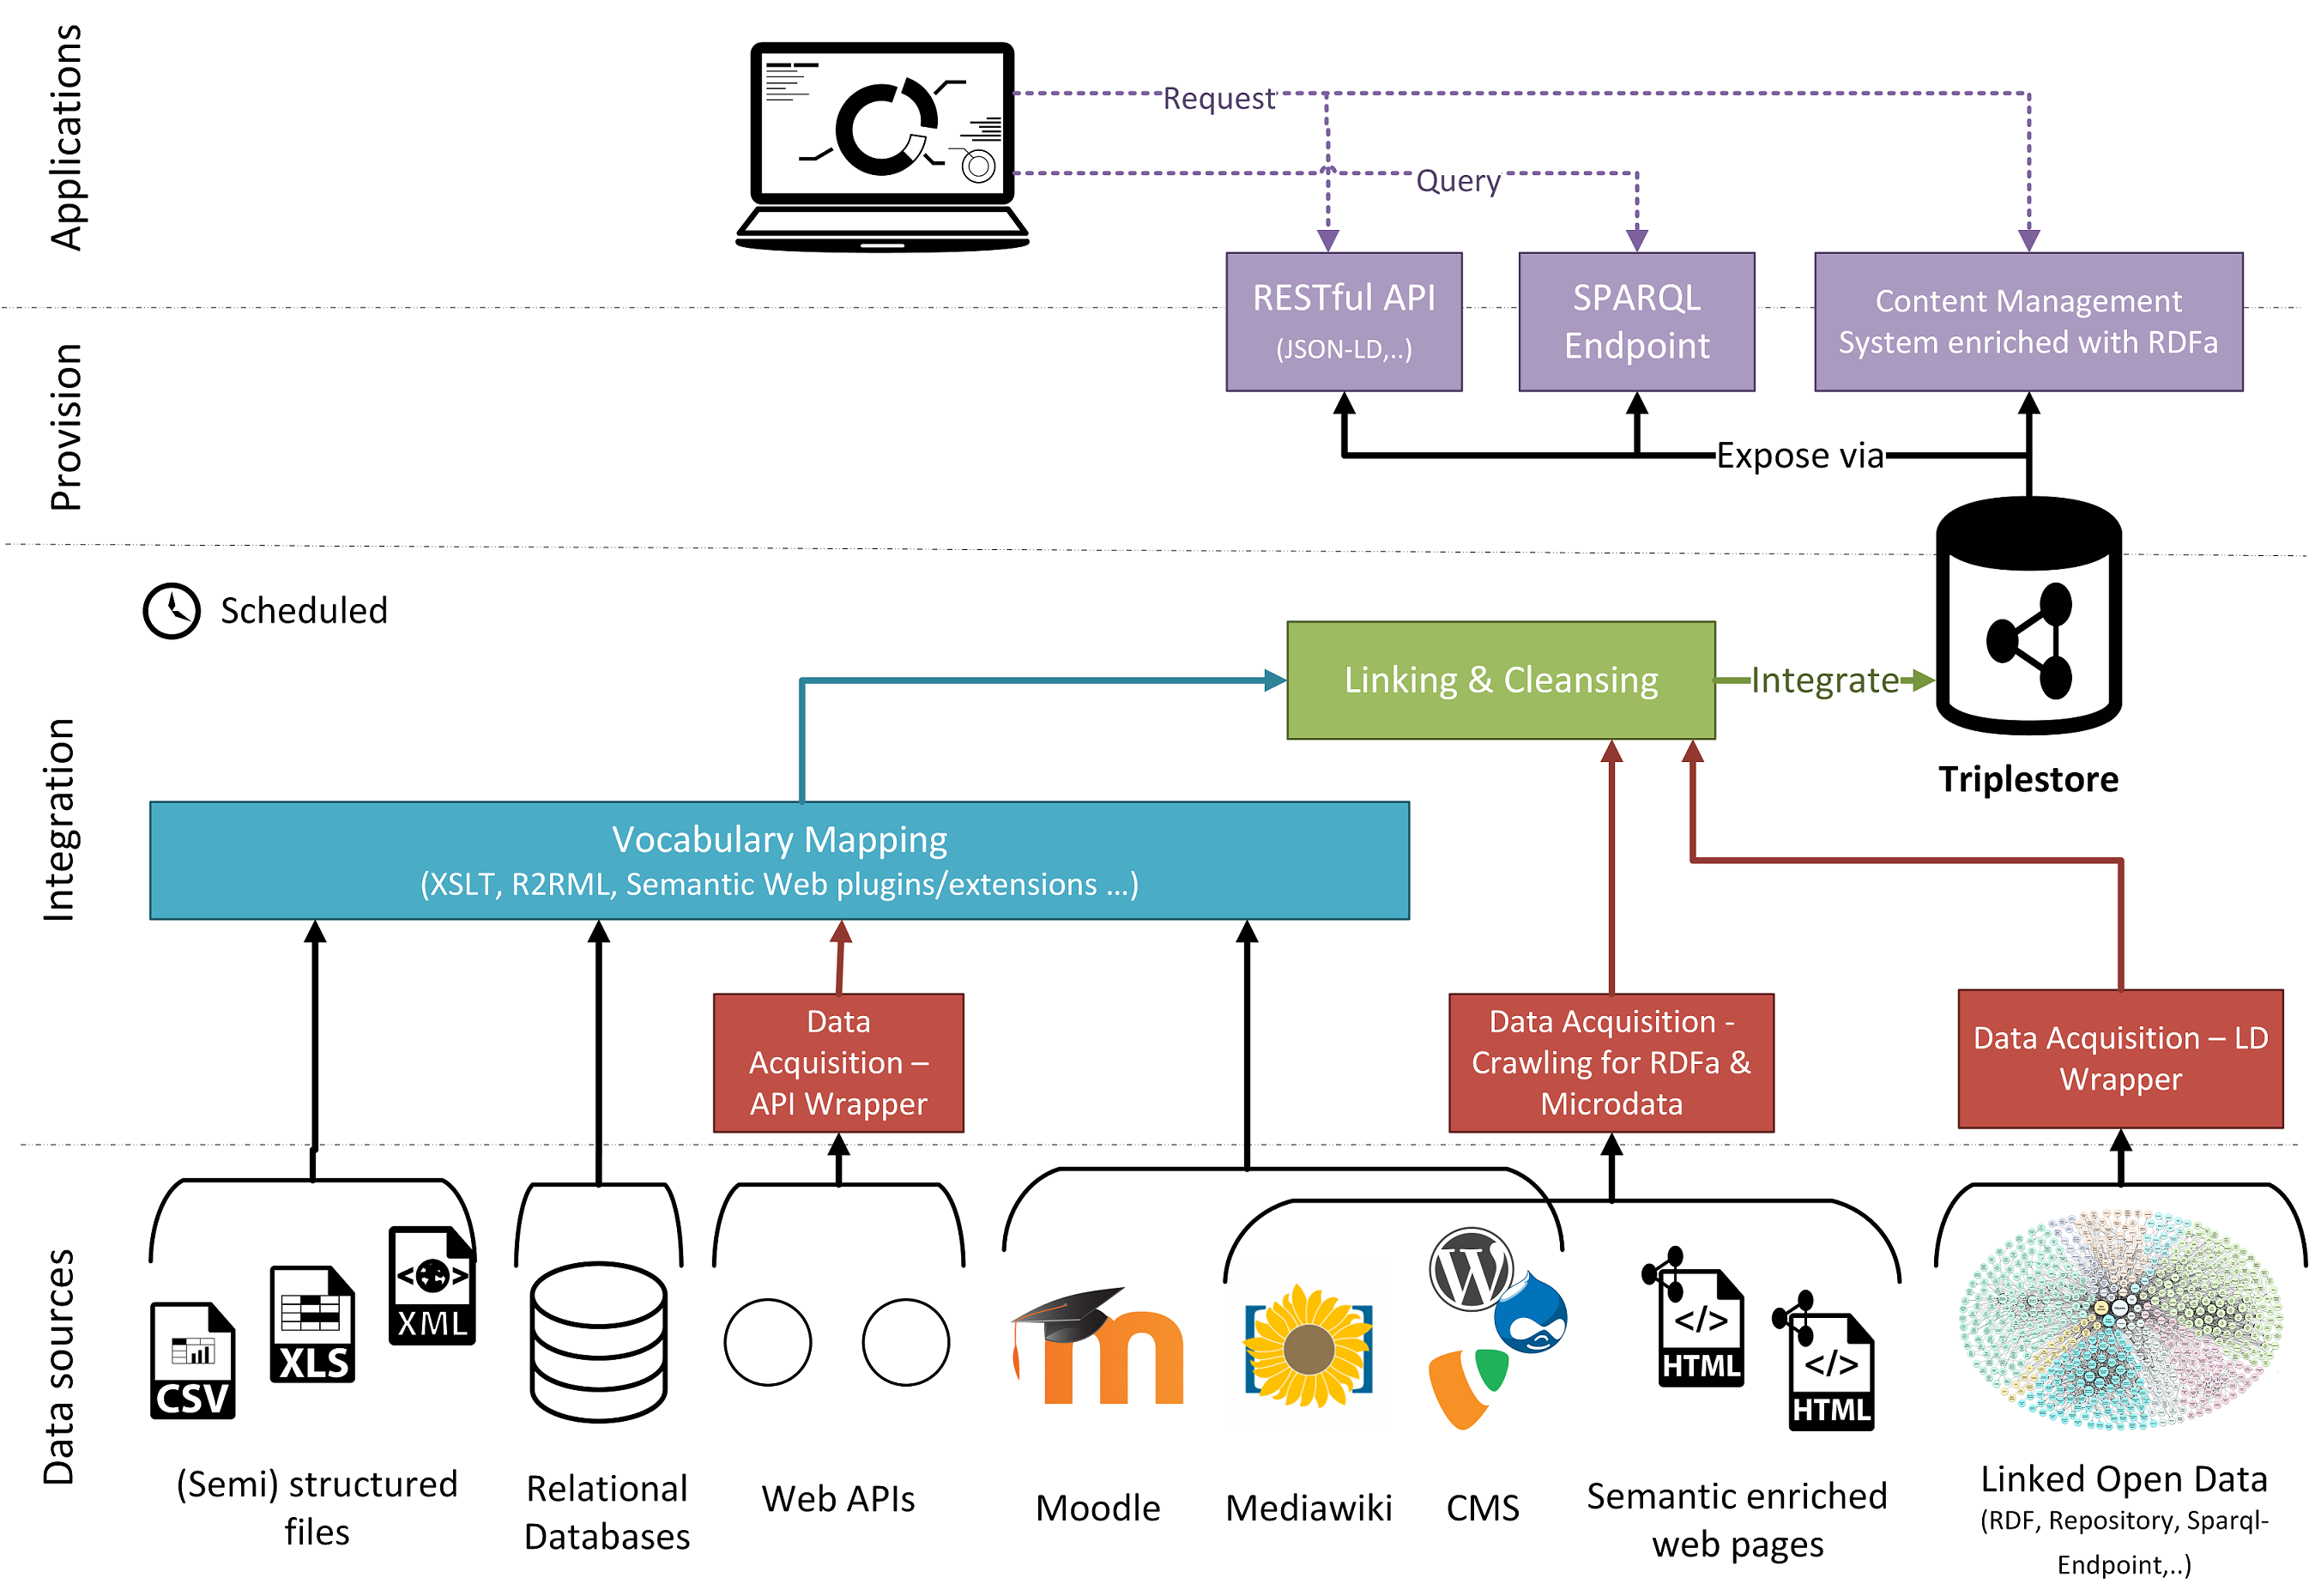
\includegraphics{images/architecture/lod_technical_architecture.png}}}
\caption[Generic high level technical architecture of a LOD system]{Generic high level technical architecture for providing Linked Open Data (adapted from EUCLID {\cite{simperl_using_2013}})}
\label{Fi:tec_architecture}
\end{figure}

\begin{figure}[htbp]
\centering
{\scalebox{0.13}{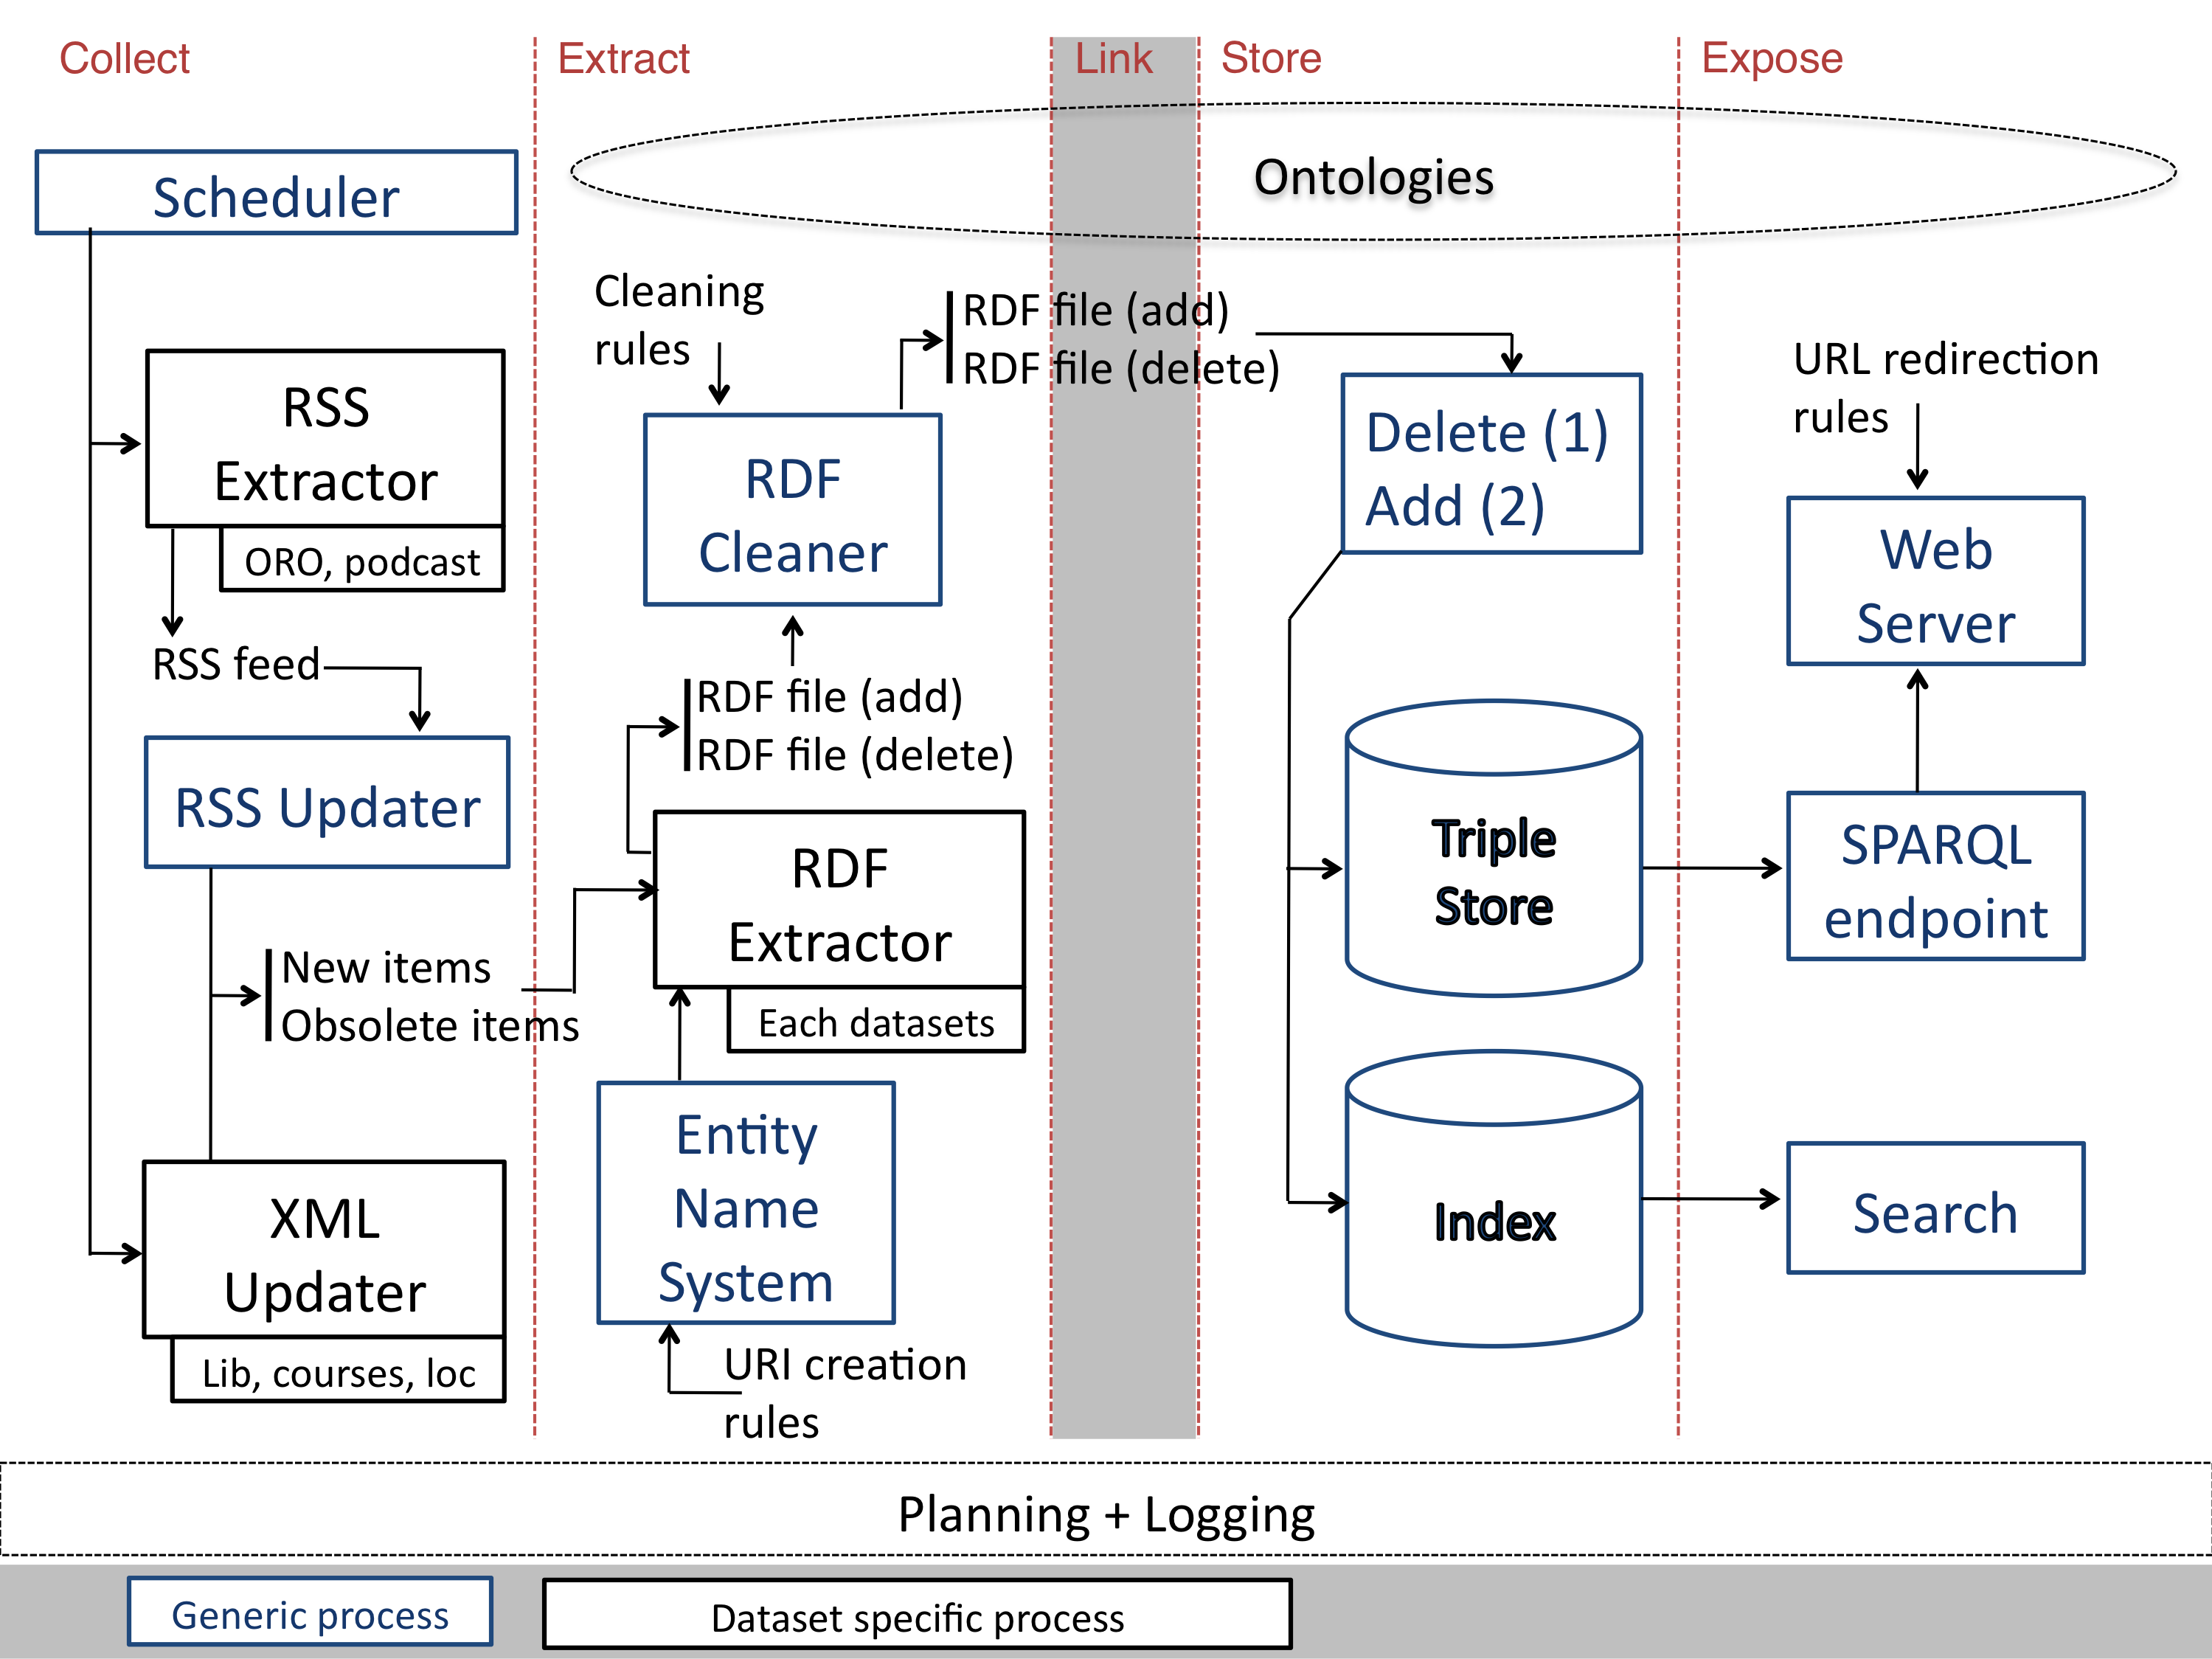
\includegraphics{images/architecture/lucero-workflow.png}}}
\caption[Example: the LUCERO workflow]{Example: the LUCERO workflow\footnote{\citet{url:lucero-tabloid}}}
\label{Fi:lucero_architecture}
\end{figure}

\subsubsection{Collect \& extract data from sources}\label{subsubsec:sources}
The first step must be to collect and extract the data from the source and transform them into a proper LOD format, e.g. RDF. By now there are basically for every data format tools for transforming them into RDF, LinkedUniversities made a collection of them~\footnote{\url{http://linkeduniversities.org/lu/index.php/tools/index.html}}, here are the main tools:

\begin{itemize}
	\item \texttt{From Relational Databases}
	\begin{itemize}
		\item \texttt{Triplify}~\footnote{\url{http://triplify.org/}} is a tool which use SQL queries to generate RDF data from a relational database.
		\item \texttt{D2RQ}~\footnote{\url{http://www4.wiwiss.fu-berlin.de/bizer/d2r-server/}} is a tool which also use SQL queries but with the use of a mapping that relates the structure of a database to RDF triples. It transformers SPARQL queries at run-time into SQL queries using this mapping.
	\end{itemize}
	\item \textbf{From XML and RSS}\newline
	In terms of syntax, XML, RSS and RDF sharing the same base, so there have to be fewer effort to be done to transform them syntactic, commonly using XSLT. W3C recommended the \texttt{GRDDL}~\footnote{\url{http://www.w3.org/TR/grddl/}} language for this purpose.
	\item \textbf{From Tables and Spreadsheets}
	\begin{itemize}
		\item \texttt{Google Refine}~\footnote{\url{http://code.google.com/p/google-refine/}} with the RDF Extension~\footnote{\url{http://lab.linkeddata.deri.ie/2010/grefine-rdf-extension/}} is an easy way to clean, transform and explore data in a tabular format including MS Excel, Google Spreadsheet and CSV.
		\item Other tools like \texttt{Any23}~\footnote{\url{http://lab.linkeddata.deri.ie/2010/grefine-rdf-extension/} (at the moment of the work unavailable)} or \texttt{QUIDICRC}~\footnote{\url{http://any23.org/}(at the moment of the work unavailable)} providing simple transformation from CSV to RDF
	\end{itemize}
\end{itemize}

After extracting the data as RDF from there source, they need to be cleaned and interlinked with themselves and other data.

\subsubsection{Vocabularies and Ontologies}\label{subsubsec:ontologies}
To represent and store the collected data, they must be mapped into an ontology and a vocabulary.

\citet{jour:gruber} defines an \textit{ontology} as ``\textit{an explicit specification of a conceptualization}''.
\textit{Conceptualizations} are objects, entities or concepts that may or may not exist in the universe. In addition to that, the \textit{vocabulary} defines the relationships between those objects. In other words, the vocabulary defines the conceptual model of what can be represented. 
\citet{jour:owl} describe ontologies from a more practical point of view defining the three conceptual components of an ontology - \textit{classes}, \textit{instances} and \textit{properties}. Regardless of what concrete implementation of an ontology is used graphical representations~(e.g. graph) are preferred over textual ones to give a high level overview of the concepts used in an ontology. 

Again, LinkedUniversities listed a lot of useful vocabularies and ontologies on their website~\footnote{~\url{http://linkeduniversities.org/lu/index.php/vocabularies/index.html}}. As an example for such an ontology let's take a look at the use case ``publication database'' from section~\ref{section:pub_db_usecase}. To mapping the data from this database a bibliographic ontology is needed. LinkedUniversities recommend the \texttt{BIBO} (Bibliographic Ontology)~\footnote{~\url{http://bibliontology.com/}}. It can be used as a citation ontology, as a document classification ontology, or simply as a way to describe any kind of document in RDF, so it is ideally for this purpose. You can see the \texttt{BIBO} graph in figure~\ref{Fi:bibo_graph}.

\begin{figure}[htbp]
\centering
{\scalebox{0.4}{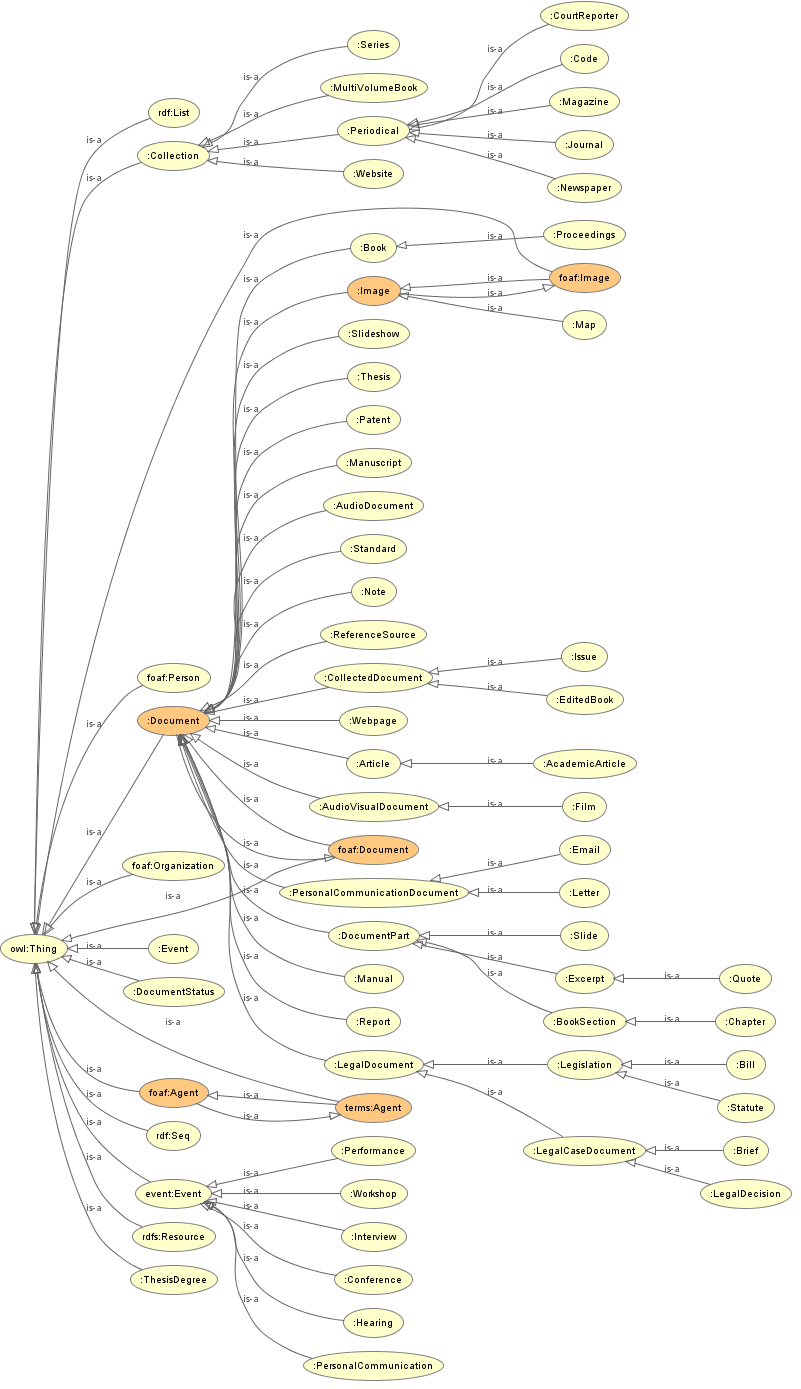
\includegraphics{images/architecture/bibo_graph_2.png}}}
\caption[BIBO graph]{Graph of the Bibliographic Ontology}
\label{Fi:bibo_graph}
\end{figure}

%\subsubsection{Link the data}\label{subsubsec:link_data}
%Another crucial element concerns the way the different datasets connect to each other. 
\subsubsection{Store the data}\label{subsubsec:store}
Considering the performance of such a system and to avoid too much communication with the original data source, the center of the system is a triple store, where the extracted data are stored and from there exposed to the web. A triple store (or RDF store) is a purpose-built database, \textit{``designed to store and retrieve identities that are constructed from triplex collections of strings (sequences of letters). These triplex collections represent a subject-predicate-object relationship that more or less corresponds to the definition put forth by the RDF standard.''}~\citet{url:triplestore}. There are a lot of implementations of such a triple store, like 
\texttt{Sesame}~\footnote{\url{http://rdf4j.org/}}, 
\texttt{Jena TDB}~\footnote{\url{http://openjena.org/TDB/}}, 
\texttt{4Store}~\footnote{\url{http://4store.org/}} or 
\texttt{SwiftOWLIM}~\footnote{\url{http://www.ontotext.com/owlim/}}. The LUCERO project settled for the \texttt{SwiftOWLIM}, because it is ``\textit{free, scalable and efficient, and includes limited reasoning capabilities, which might end up being useful in the future}''~\citet{url:lucero-tabloid}.

\subsubsection{Expose the data to the Web}\label{subsubsec:provision}
The last step is obviously to expose the data from the triple store to the web. For this purpose a SPARQL endpoint is commonly used, but there are also other way, e.g. resolvable URIs, the linked data API~\footnote{\url{http://code.google.com/p/linked-data-api/}} or an Open RESTful API. All of them make the data available so others can query and access them to use it for their application or to serve themselves as resource for linking it with other data.

%\subsection{Stakeholder specific issues (datasets, application types)}
\subsection{Challenges}
In this section we will briefly describe some of the most crucial factors which has to be faced when implementing a system similar to the proposed one.

\subsubsection{Data ownership}
When exposing data as LOD the ownership of the original data has to be cleared without any doubt, so there are no legal concerns to be cared about when implementing the system. An unclear ownership may otherwise lead to a complete failure of the project, if the worst comes to the worst at a time where already a lot of time and work are spent. Further, to ensure a stable system, the ownership has be clear over a long time in the future - otherwise other applications, built on the data, loose their source.

\subsubsection{Data quality}
Publishing a LOD system there must be a compromise found between actuality of the data and a proper system load of the interface to the data source (e.g. an active used database), so existing system may not be (to heavily) effected by the LOD system. According to the data the actuality may range between weeks and days (e.g. for location data) or minutes and seconds (e.g. public transport data).

Further it must be ensured that the linking of the data are valid at every time, linking to no longer existing sources or sources with sinking data quality will lower the quality of data itself.

\subsubsection{Response time of the LOD interface}
To achieve not only a providing of the data but also a use of the data in applications, the interface (e.g.